%% content.tex
%%


%% ===========================
\chapter{Umsetzung}
\label{ch:umsetzung}
%% ===========================

In diesem Kapitel wird auf die Implementierung der Konzepte eingegangen. Die Architektur wurde wie in der Konzeption beschrieben umgesetzt. Daher wird vielmehr auf die genauen Funktionsweisen und Prozesse eingegangen. Anhand von Klassendiagrammen wird in den ersten beiden Kapiteln die Struktur und Funktionsweise der Webprojekte erläutert. Weiterhin wird der ETL-Prozess und die Abfrageerzeugung detailliert beschrieben. Der genaue Ablauf in der Aktualisierung wird in dem darauf folgenden Abschnitt behandelt. Abschließend wird der Aufbau der Oberfläche mit den damit verbundenen Designentscheidungen erläutert. 

%% ===========================
\section{Server-Webprojekt}
%% ===========================

Es handelt sich um ein dynamisches, Java-basiertes Eclipse-Webproject, dessen Struktur und Einstellungen den Standardvorgaben aus der Erzeugung entsprechen. Deshalb wird direkt auf die Klassen eingegangen. Abbildung \ref{umsetzung_klassendiagramm_server} zeigt das Klassendiagramm des Server-Webprojekt. Das Diagramm dient als Basis für die nachfolgenden Erläuterungen. 

Die H2-Datenbank wird im Embedded-Modus betrieben, was eine Instanziierung der Datenbank zur Laufzeit notwendig macht. Die Instanziierung erfolgt in der Klasse \textit{Database}. Das Attribut \textit{dataSource} stellt die H2-Datenbank in Form eines Objektes dar. Eine Verbindung zur Datenbank wird mithilfe der Methode \textit{getConnection()} aufgebaut. Diese Verbindung wird permanent offen gehalten, solang der Tomcat-Server läuft. Dazu wird die Verbindung dem Attribut \textit{con} zugewiesen, welches von allen Methoden verwendet wird, die eine Verbindung zur Datenbank aufbauen wollen. Um die Datenbank mit der Web-Anwendungen zu starten, ist die Verwendung eines Servlets nötig. Dazu benutzen wir die Klasse \textit{EntryPoint}, die das Interface \textit{HttpServlet} implementiert. Um das Servlet direkt beim Start des Tomcats aufzurufen, sind in der \textit{web.xml} folgende Zeilen eingetragen: 

\begin{lstlisting}[language=XML]
	<servlet>
		<servlet-name>H2</servlet-name>
		<servlet-class>de.cas.db.EntryPoint</servlet-class>
		<load-on-startup>1</load-on-startup>
	</servlet>
\end{lstlisting}

Die 1 im Element \textit{<load-on-startup>} bewirkt den Aufruf der Methode \textit{init()} die eine Instanziierung der Klasse \textit{Database} vornimmt. Zur Erzeugung des Schemas wird eine separate Klasse namens \textit{SchemaBuilder} eingesetzt. In ihr werden sämtliche SQL-Anweisungen zur Generierung des Schemas aufbewahrt und können über die Methode \textit{createSchema()} ausgeführt werden.

\begin{figure}[htbp]
\begin{center}
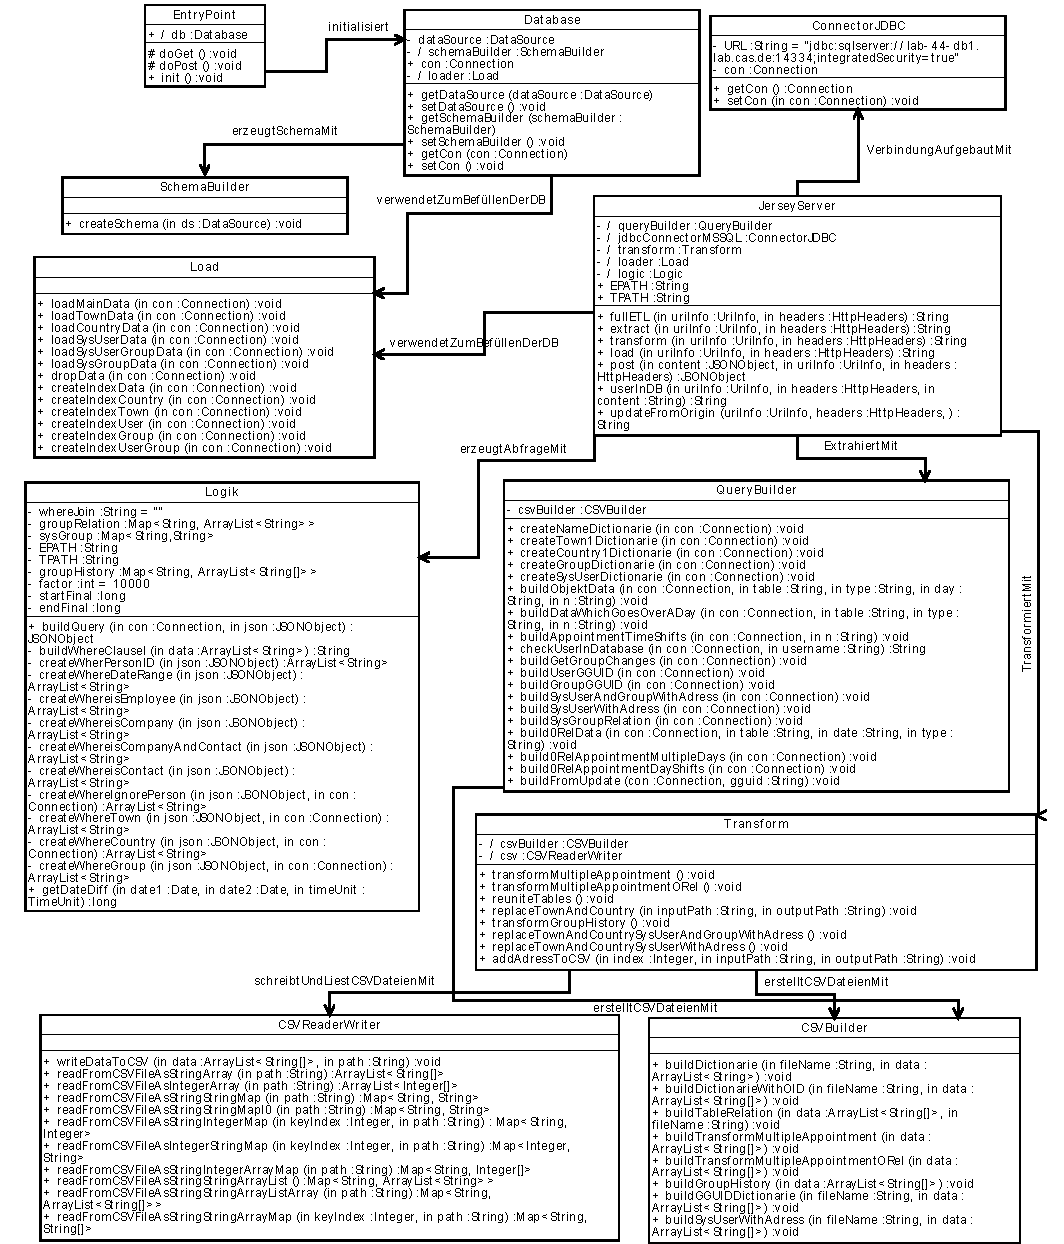
\includegraphics[width=1.0\textwidth]{pics/ServerKlassendiagramm.pdf}
\caption{Server Klassendiagramm}
\label{umsetzung_klassendiagramm_server}
\end{center}
\end{figure}

In der Klasse \textit{JerseyServer} ist ein REST-Server implementiert. Sie besitzt Methoden die mit den entsprechenden Annotationen, wie \textit{@GET} oder \textit{@POST}, die REST-Requests entgegen nehmen. Mit der Annotation \textit{@Path} wird die URL angegeben, unter der die Methode angesprochen werden kann. Diese Methoden besitzen Übergabeparameter vom Typ \textit{UriInfo} und \textit{HttpHeaders} besitzen, mithilfe denen die Metadaten der REST-Requests abgegriffen werden. 

Neben den Methoden zur Verarbeitung von REST-Requests, enthält die Klasse alle Objekte zur Durchführung des ETL-Prozesses. Das Objekt  \textit{ConnectorJDBC} besitzt ein Attribut namens \textit{con}, welches den Verbindungsaufbau zum MSSQL-Server, mithilfe von JDBC ermöglicht. Zur Extraktion der Daten aus der MSSQL-Datenbank wird ein Objekt der Klasse \textit{QueryBuilder} verwendet. Wie in der Abbildung zu sehen wird für jede SQL-Anweisung eine eigene Methode mit den entsprechenden Konfigurationen verwendet. Methoden welche die Übergabewerte \textit{table}, \textit{date} und \textit{n} besitzen, werden zum Beschaffen der CRM-Objekte eingesetzt. Mithilfe des Parameters \textit{table} wird der betroffene Tabellenname aus der MSSQL-Datenbank übergeben. Der Parameter \textit{date} gibt das Attribut an, was für die Ermittlung des Datums verwendet werden soll. Um den Typ eines CRM-Objektes zwischen Personen festzuhalten wird der Parameter \textit{n} verwendet, der eine Zahl zwischen eins und fünf beinhaltet. \textit{QueryBuilder} verwendet ein Objekt der Klasse \textit{CSV-Builder}, um die Ergebnisse der SQL-Abfragen in Dateien festzuhalten. Den Methoden wird als Übergabeparameter ein Dateiname sowie die zu speichernden Informationen übergeben.

Die Klasse \textit{Transform} enthält Attribute und Methoden zur Bearbeitung der in der Extraktion erzeugten CSV-Dateien. Der Inhalt der Dateien wird mithilfe eines \textit{CSVReaderWriter} Objekts ausgelesen und in die Java-Laufzeitumgebung geladen. Nach der Bearbeitung durch die Methoden der \textit{Transform} Klasse, werden die Daten wieder in CSV-Dateien zurückgeschrieben. \textit{CSVBuilder} besitzt Methoden die zusätzliche Parameter zum Schreiben aufweisen, die spezielle Schreiboperationen erlauben. Wohingegen \textit{CSVReaderWriter} mithilfe der Methode \textit{writeDataToCSV()}, sowie den Parametern \textit{path} und \textit{data} für allgemeine Schreiboperationen verwendet wird.

Mithilfe der Klasse \textit{Load} wird die Datenbank befüllt. Sie wird von den \textit{Database} und \textit{JerseyServer} Objekten verwendet. In der Klasse \textit{JerseyServer} werden mit der Methode \textit{load()} die Methoden der Klasse \textit{Load} aufgerufen. In der Klasse \textit{Database} werden sie im Konstruktor selbst aufgerufen, um die Datenbank beim starten des Anwendungsserver automatisch zu befüllen. 

Die Klasse \textit{Logik} beinhaltet Attribute und Methoden zum beantworten von Benutzerabfragen. Für jede Bedingungen der SQL-Abfrage an die H2-Datenbank wird eine separate Methoden verwendet. Die jeweiligen Methoden werden nur gerufen, sobald der entsprechende Eintrag in der vom Benutzer übermittelten JSON-Datei vorhanden ist. Generiert werden die Abfragen an die H2-Datenbank durch die Methode \textit{buildQuery()}. 

%% ===========================
\section{Client-Webprojekt}
\label{ch:Umsetzung:sec:clientwar}
%% ===========================

Der Einstiegspunkt des Webprojekts ist die Klasse \textit{CasAnalyticUI}. Sie ist von der Vaadin-Klasse \textit{UI} abgeleitet. Die \textit{UI} ist die oberste Komponente jeder Komponentenhierarchie in Vaadin. Es gibt eine Benutzeroberfläche für jede Vaadin-Instanz in einem Browserfenster. Ein \textit{UI} Objekt kann entweder ein gesamtes Browserfenster(oder Tab) oder einen Teil einer HTML-Seite, wo eine Vaadin-Anwendung eingebettet ist darstellen. Nachdem eine \textit{UI} von der Anwendung erstellt wurde, wird diese mit der Methode \textit{init(VaadinRequest)} initialisiert. Zur Übersicht sind die Komponenten der Darstellung in die Klasse \textit{RootUI} ausgelagert. 

Die \textit{RootUI} wird in der \textit{CasAnalayticUI} instanziiert. Die Klasse \textit{RootUI} beinhaltet Objekte die Vaadin-Komponenten zur Darstellung des Anmeldefensters sowie der Hauptansicht. Mithilfe der Methode \textit{buildLoginView()} werden die Komponenten des Anmeldefensters zur \textit{UI}-Komponente hinzugefügt. Nach der Erzeugung der Komponenten, wird eine \textit{JerseyClient} Klasse instanziiert. Diese wird verwendet sobald der Nutzer IP, Port und einen Namen eingegeben hat und auf anmelden klickt. Anschließend wird die Methode \textit{doPostRequestUserData()} gerufen, um zu überprüfen ob der Nutzer im System vorhanden ist. 

Falls ja, werden durch die Methode \textit{MainView()} alle bisherigen Komponenten der \textit{UI} entfernt und durch Komponenten des Hauptfensters ersetzt. Das \textit{JerseyClient} Objekt wird direkt im Anschluss verwendet, um mithilfe der Methode \textit{doPostRequestData()} einen REST-Request an den Server zu senden. Dieser liefert das Ergebnis der SQL-Abfrage in einem JSON-Objekt zurück, mit dessen eine erste Erzeugung des Diagramms durchgeführt wird. Das Diagramm selbst besitzt eine eigene Klasse namens \textit{ChartComponent}. Sie leitet sich von der Klasse \textit{Chart} ab, die Teil der VaadinChart-Bibliothek ist. Mithilfe der Methode \textit{refreshChart()} wird das Diagramm bei Benutzerabfragen aktualisiert. Dazu werden ihr die Namen der Personen für die x-Achse übergeben sowie die neuen Balkenwerte. Weiterhin wird für jede Vaadin-Komponente eine separate Methode zur Konfiguration verwendet. Änderungen am Aussehen oder an der Funktionalität der jeweiligen Vaadin-Komponenten, werden nur innerhalb der entsprechenden Methode vorgenommen.

\begin{figure}[htbp]
\begin{center}
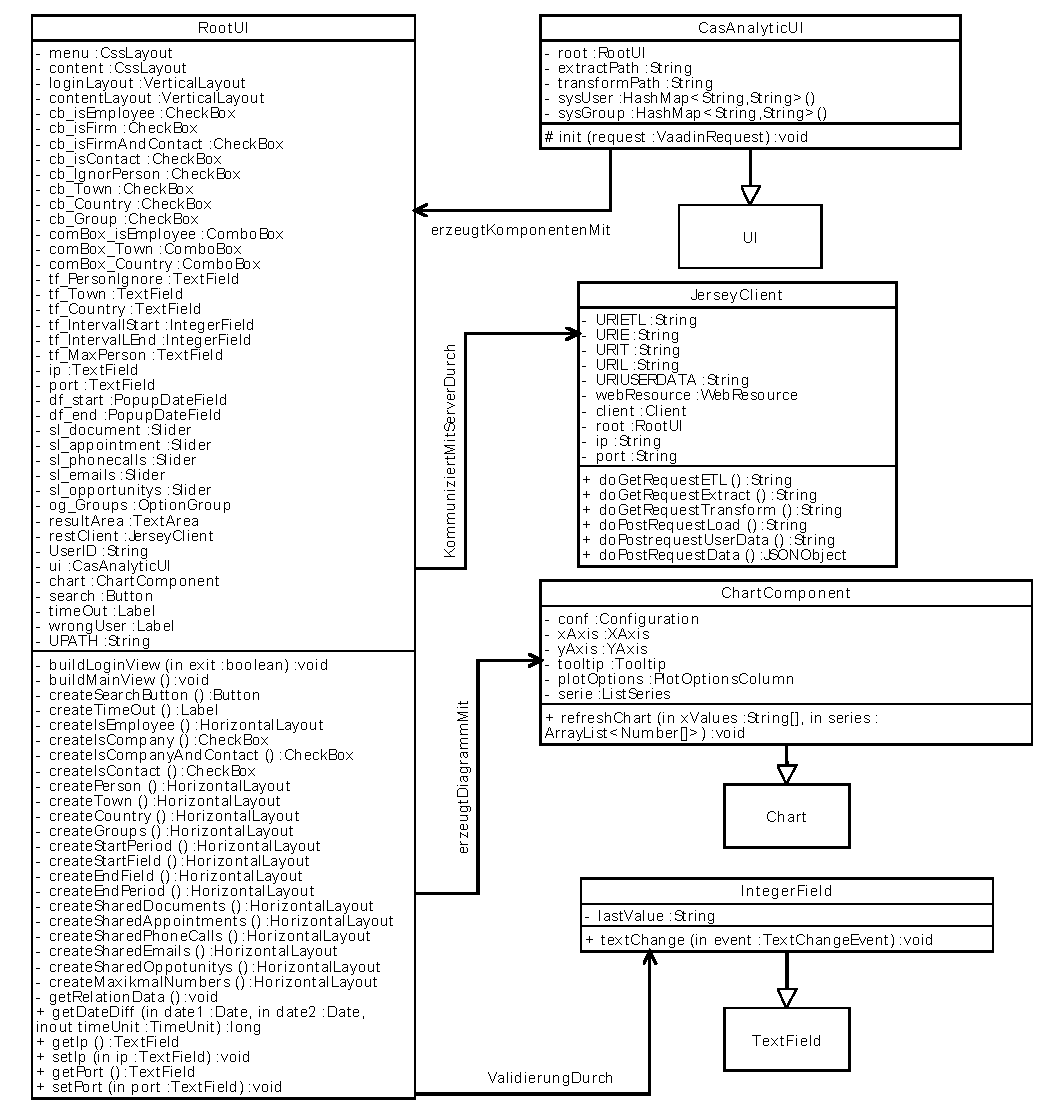
\includegraphics[width=0.9\textwidth]{pics/ClientKlassendiagramm.pdf}
\caption{Client Klassendiagramm}
\label{umsetzung_klassendiagramm_client}
\end{center}
\end{figure}

An der Oberfläche gibt es Eingabefelder die nur Zahlen erwarten. Eingaben die nicht numerisch sind werden durch den Einsatz der Klasse \textit{IntegerField} verhindert. Diese erweitert die Klasse \textit{TextField}. Sie besitzt einen Event-Listener, der jede Eingabe des Benutzers abfängt. Gibt der Nutzer nicht numerische Zeichen ein werden diese direkt wieder entfernt. Dadurch werden Falscheingaben durch den Nutzer ausgeschlossen.

%% ===========================
\section{Aufbau der H2-Datenbankabfrage}
%% ===========================

Um eine SQL-Abfragen möglichst schlank zu halten werden Teile der SQL-Anweisung nur bei entsprechenden Eingaben der Benutzer verwendet. Die SQL-Abfrage kann dadurch je nach Benutzereingabe unterschiedlich aufgebaut sein kann. Die Basisfunktionalität ändert sich allerdings nicht. Diese besteht aus der Bildung von Summen der verschiedenen CRM-Objekte. Nachdem festgestellt wurde wie viele CRM-Objekte von den jeweiligen Typen zu einer Person verlaufen, wird zusätzlich die Gesamtsumme der CRM-Objekte zu einer Person gebildet. Die Summe wird zur Sortierung der Ergebnisse verwendet. Bei der Sortierung wird absteigend vorgegangen, um die Personen mit den meisten CRM-Objekten zu der von der Suche ausgehend Person zu ermitteln. Das Ergebnis wird wiederum auf eine durch den Benutzer festgelegte Anzahl reduziert. Überdies beschränkt die SQL-Anweisung den Zeitraum der Analyse.

Eine weiterer Bestandteil der SQL-Anweisung ist die Gewichtung von Zeitspannen. Das Verfahren zur Gewichtung der Zeit wird anhand der Abbildung \ref{fig:umsetzung:gewichtungderzeit} erläutert. Die Abbildung zeigt ein Koordinatensystem mit der Gewichtung von einzelnen Zeitpunkten. Die x-Achse stellt den zeitlichen Verlauf und die y-Achse die Gewichtung dar. Der Startzeitpunkt wird durch $t_{s}$ markiert, wohingegen $t_{e}$ den Endzeitpunkt angibt. Mithilfe von $t_1$ und $t_2$ werden die zu gewichtenden Zeitspannen festgelegt. Um nun die Zeitspannen anders zu gewichten wird eine lineare Abstufung der Tage vorgenommen. Für die Zeitspanne zwischen $t_{s}$ und $t_1$ bedeutet dies, dass der Wert eines Tages zunehmend steigt. Wird $t_1$ erreicht, besitzt jeder Tage wieder eine Wertigkeit von 1. Bei $t_2$ verhält es sich ähnlich. Mit jedem Tag ab $t_2$ sinkt der Wert des Tages bis der Zeitpunkt $t_{e}$ erreicht ist.

Um die Gewichtung eines bestimmten Tages zu berechnen werden die folgenden zwei Faktoren verwendet:

\begin{equation}
f_1 = \frac{1}{t_1 - t_{s}}
\end{equation}
\begin{equation}
f_2 = \frac{1}{t_{e} - t_2}
\end{equation}

Neben den Faktoren $f_1$ und $f_2$ werden Variablen zum erfassen der schrittweisen Erhöhungen und Verringerungen von Tagen benutzt. Für den Zeitraum zwischen   
$t_{s}$ und $t_{1}$ wird die Variable $v_{1}$ verwendet. Der andere Zeitraum arbeitet mit der Variable $v_{2}$. Die Variable $v_{1}$ beginnt mit dem Wert 0 und erhöht sich mit jedem Tag um 1. Die Differenz zwischen $t_{2}$ und $t_{e}$ stellt den Wert von $v_{2}$ dar. Dieser wird mit jedem Tag ab $t_{2}$ um 1 verringert.

Mit den Faktoren und Variablen werden die Werte der Tage berechnet. Dazu wird der Faktor mit der Variabel multipliziert. Das Produkt bildet den Wert eines Tages. Dieser wird in der Datenbankabfrage verwendet, um Tupeln einen geringeren Wert zuzuweisen. 

\begin{figure}[htbp]
\begin{center}
\begin{tikzpicture}[domain=-1:2] \draw[very thin,color=gray] (0,0); 
\draw[->] (0,0) -- (12.3,0) node[right] {Zeit}; 
\draw[->] (0,0) -- (0,4.2) node[above] {Gewichtung}; 
\draw[color=black]  (0.2,3) -- (-0.2,3)   node[left] {100\%};
\draw[color=black]  (0.2,1.5) -- (-0.2,1.5)   node[left] {50\%};  
%\draw[dashed][color=black]  (4,0.5) -- (4,3.5); 
%\draw[dashed][color=black]  (9,0.5) -- (9,3.5);

\draw[color=black]  (0,0) -- (0,0)   node[below] {$t_{s}$}; 
\draw[color=black]  (4,0.1) -- (4,-0.1)   node[below] {$t_1$}; 
\draw[color=black]  (9,0.1) -- (9,-0.1)   node[below] {$t_2$};
\draw[color=black]  (12,0.1) -- (12,-0.1)   node[below] {$t_{e}$};   
 
\draw[color=black]  (0,0) -- (4,3)   node[right] {}; 
\draw[color=black]  (4,3) -- (9,3)   node[right] {}; 
\draw[color=black]  (9,3) -- (12,0)   node[right] {};  

\draw[dotted][color=black]  (1,0.75) -- (2,0.75);
\draw[dotted][color=black]  (2,1.5) -- (3,1.5);
\draw[dotted][color=black]  (3,2.25) -- (4,2.25);
\draw[dotted][color=black]  (4,3) -- (5,3);

\draw[dotted][color=black]  (1,0.75) -- (1,0);
\draw[dotted][color=black]  (2,1.5) -- (2,0);
\draw[dotted][color=black]  (3,2.25) -- (3,0);
\draw[dotted][color=black]  (4,3) -- (4,0);
\draw[dotted][color=black]  (5,3) -- (5,0);
\draw[dotted][color=black]  (6,3) -- (6,0);
\draw[dotted][color=black]  (7,3) -- (7,0);

\draw[dotted][color=black]  (8,3) -- (8,0);
\draw[dotted][color=black]  (9,3) -- (9,0);
\draw[dotted][color=black]  (10,2) -- (10,0);
\draw[dotted][color=black]  (11,1) -- (11,0);

\draw[dotted][color=black]  (8,3) -- (9,3);
\draw[dotted][color=black]  (9,2) -- (10,2);
\draw[dotted][color=black]  (10,1) -- (11,1);

\draw[dashed][color=black]  (1,0.75) -- (1,1.05)   node[above] {$t_{s}+1$}; 
\draw[dashed][color=black]  (2,1.5) -- (2,1.8)   node[above] {$t_{s}+2$}; 
\draw[dashed][color=black]  (3,2.25) -- (3,2.55)   node[above] {$t_{s}+3$};  

\draw[dashed][color=black]  (10,2) -- (10,2.3)   node[above] {$t_{e}-2$}; 
\draw[dashed][color=black]  (11,1) -- (11,1.3)   node[above] {$t_{e}-1$}; 

\end{tikzpicture} 
\end{center}
\caption{Gewichtung der Zeit}
\label{fig:umsetzung:gewichtungderzeit}
\end{figure}

Neben der Zeit lassen sich die jeweiligen CRM-Objekte unterschiedlich gewichten. Bei einer Abweichung von 100 Prozent wird die Anzahl des jeweiligen CRM-Objektes, um den entsprechenden Prozentsatz verringert. 

Die restlichen vom Benutzer festgelegten Parameter fügen weitere Bedingungen in die SQL-Anweisung ein. Eine muss zuvor ermittelt werden und wird daher näher beschrieben. Es handelt sich dabei um Gruppen, die aus der Ergebnismenge ausgeschlossen werden können. Ihre Konstellation in Bezug auf Personen ist im Laufe der Zeit variabel. Um dies zu berücksichtigen wird die Tabelle \textit{UserGroup} verwendet. Dabei wird folgendermaßen vorgegangen: Zuerst wird für jede Gruppe ein eigener Container erzeugt. Der Container beinhaltet die IDs der Personen aus der Gruppe. Liegt nun der Zeitpunkt des Feldes \textit{Date} nach dem Anfangszeitpunkt der Abfrage und die Spalte \textit{Action} enthält eine 1, wird der Container um diese Person reduziert. Enthält sie eine 0, wird die Person zum Container hinzugefügt. Mit einer 1 in der Spalte \textit{Action} wird der Austritt einer Person aus der Gruppe markiert. Eine 0 weist auf den Eintritt einer Person in die Gruppe hin. Dadurch wird die Struktur der Gruppe zum Anfangszeitpunkt wiederhergestellt. Mithilfe des Containers wird anschließend die SQL-Anweisung um weitere auszuschließende Personen erweitert.

Innerhalb von Zeiträumen können sich Gruppen auch verändern, jedoch kann dies nicht berücksichtigt werden. Es kann jeweils nur ein bestimmter Zeitpunkt betrachtet werden. In unserem Fall entschied man sich für den Anfangszeitpunkt $t_{s}$.

%% ===========================
\section{ETL-Prozess}
%% ===========================

Zuerst wird auf die Schritte in der Extraktion eingegangen. Das Vorgehen hierfür ist in der Abbildung \ref{umsetzung_extract} dargestellt. Indessen wird ein Verbund gebildet, der Tupeln aus den betroffenen Tabellen verschmelzen lässt. Die Erzeuger der CRM-Objekte werden mithilfe der Tabelle \textit{TableRelation} ermittelt. Zur Ermittlung der Verknüpfungen zwischen der Person und den CRM-Objekten wird als erstes eine SQL-Anweisung verwendet, die für jede der Tabellen \textit{gwOpportunity}, \textit{gwPhoneCall0}, \textit{Document0}, \textit{EmailStore0} und \textit{Appointment0} separat ausgeführt wird. 

\begin{figure}[htbp]
\centering
  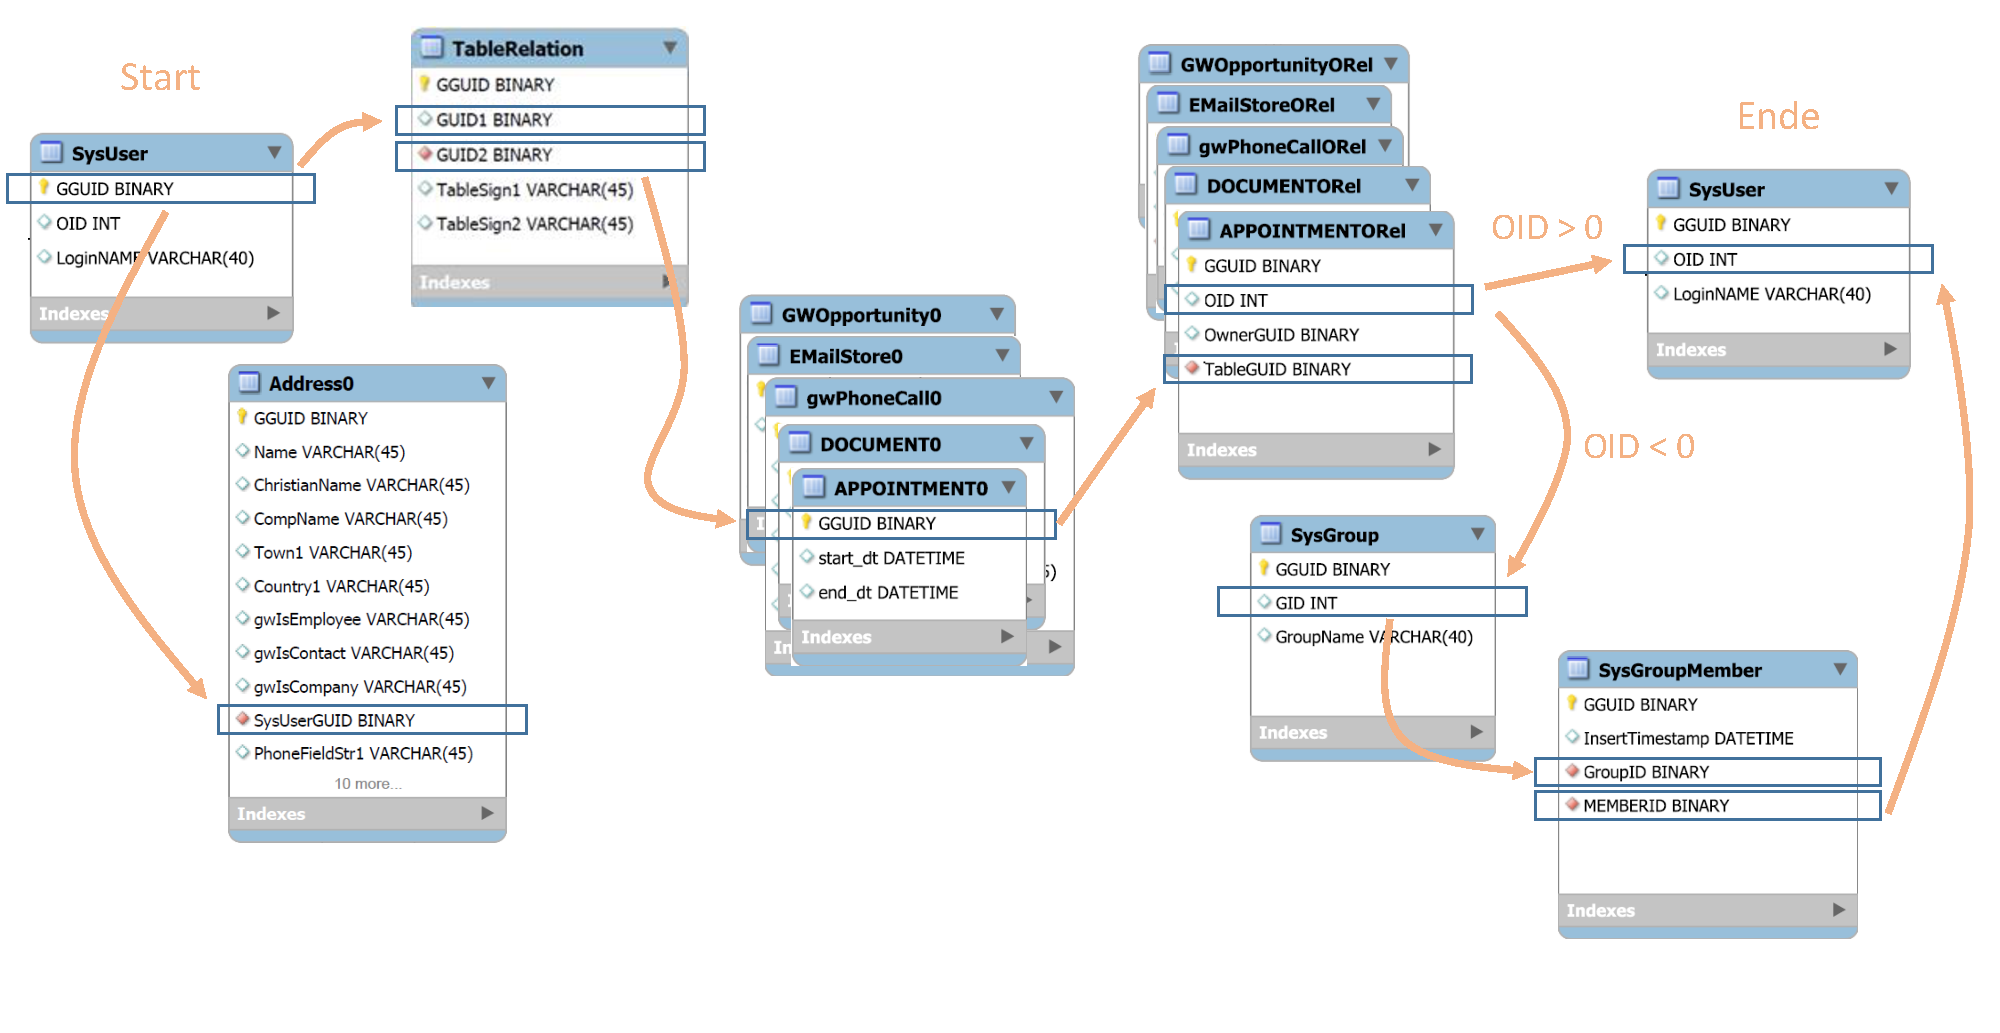
\includegraphics[width=1.0\textwidth]{pics/konzept_extraktion.pdf}
\caption{Vorgehensweise bei der Extraktion}
\label{umsetzung_extract}
\end{figure} 

Mithilfe eines Verbundes zwischen den Tabellen \textit{SysUser} und \textit{Address0} werden die Adressen der Personen ermittelt. Anschließend werden durch einen Verbund zwischen \textit{TableRelation} und \textit{SysUser} alle Tabellen ermittelt, mit denen die Personen eine Verknüpfung besitzen. Der nächste Verbund wird zwischen \textit{TableRelation} und einer der fünf zuvor genannten Tabellen gebildet. Um beispielsweise festzustellen mit welchen anderen Personen ein Dokument geteilt ist, wird ein weiterer Verbund mit der passenden ORel-Tabelle gebildet. In der ORel-Tabelle kann die \textit{OID} positiv, sowie negativ sein. Bei einem negativen Wert stellt die \textit{OID}, eine \textit{GID} der Tabelle \textit{SysGroup} dar. Zur Auflösung von Gruppen in einzelne Personen werden folgende Verbunde gebildet. Zuerst zwischen \textit{SysGroup} und \textit{SysGroupMember}, um alle Personen die zu einer Gruppe gehören zu erhalten. Anschließend zwischen \textit{SysGroupMember} und \textit{SysUser}, um die \textit{OID} der Person zu erhalten. 

Die durch den Verbund gewonnen Informationen werden weiterhin auf die 9 relevanten Werte des neuen Schemas verringert. Zu einem die \textit{OID} des \textit{SysUser}, von dem die Suche ausgeht. Zum anderen das Datum, welches durch das CRM-Objekt ermittelt wird. Weiterhin wird die zweite \textit{OID} beibehalten, die durch den Verbund mit einer zweiten \textit{SysUser} Tabelle gewonnen wird. Zum Schluss wird manuell eine vierte Information beigefügt, die besagt welchem CRM-Objekt die Tupel entstammt. Weiterhin werden die restlichen fünf Werte aus der Adresse übernommen. 

Für den Sonderfall das ein Datum über mehrere Tage geht, wird eine zehnter Wert an das Ergebnis angehängt, welche den Zeitraum in Tagen beinhaltet. Zur Beschaffung der geschobenen Termine wird genau wie in Kapitel \ref{ch:konzeption:etl:extract} beschrieben verfahren.

Jedes Ergebnis einer Datenbankabfrage wird in einer CSV-Datei direkt auf dem Tomcat-Server gespeichert. Diese CSV-Dateien stellen die Grundlage der Transformation dar. Jede dieser Dateien beinhaltet die Werte für die Tabelle \textit{Data} aus der H2-Datenbank, in der Form wie sie in Abbildung \ref{fig:umsetzung_csv_datei} zu sehen ist. 

\begin{figure}[htbp]
\begin{center}
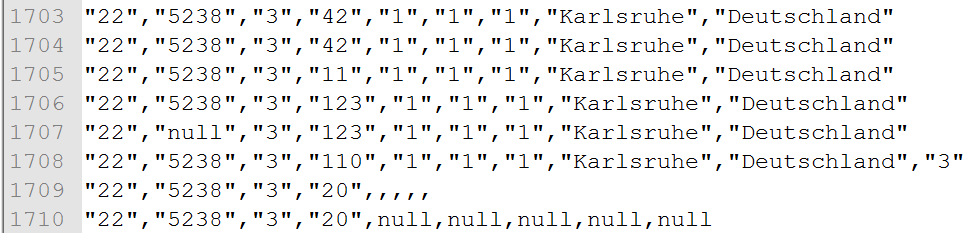
\includegraphics[width=1.0\textwidth]{pics/umsetzung_csv_datei.png}
\caption{Ausschnitt einer CSV-Datei nach der Extraktion}
\label{fig:umsetzung_csv_datei}
\end{center}
\end{figure}

Alle CSV-Dateien werden auf die in Abbildung \ref{fig:umsetzung_csv_datei} zu sehenden Anomalien untersucht. Dabei wird in Zeilen in denen die letzten fünf Werte fehlen (Zeile 1709), die Adresse über die zweite \textit{OID} ergänzt. Bei Nullwerten wird überprüft ob wirklich keine Adresse vorhanden ist, falls doch wird die Adresse ergänzt. In Zeile 1707 ist zu sehen, dass ein Nullwert anstatt eines Datum vorkommen kann. Diese Zeilen werden aus den CSV-Dateien entfernt. Wenn wie in Zeile 1708 ein zusätzlicher Wert vorhanden ist, erstreckt sich die Dauer des CRM-Objektes über mehrere Tage. Die Zeile bleibt bestehen allerdings wird der letzte Wert entfernt. Die Zahl wird jedoch zwischengespeichert und zur Erzeugung der entsprechenden Anzahl von Tupeln wiederverwendet. Bei einer Dauer von drei Tagen würde die Zahl entfernt und zwei weitere Tupeln in die Datei eingefügt werden. Jede Tupel würde einen anderen Tag in der Zeitspanne des CRM-Objektes darstellen. Nach der Beseitigung von Anomalien werden noch die Städte und Länder durch ihre jeweilige \textit{ID} aus der Tabelle \textit{Town} und \textit{Country} ersetzt.

Die überprüften Daten werden wieder in CSV-Dateien abgelegt. Diese besitzen den gleichen Namen, allerdings wird noch der Zusatz "\_transf" angehängt, der sie als transformiert kennzeichnet. Diese Dateien werden anschließend in der Java-Laufzeitumgebung zusammengeführt. Bei der Zusammenführung sind zum ersten mal alle Daten gleichzeitig in der Anwendung vorhanden, weshalb an dieser Stelle alle Duplikate beseitigt werden. Überdies werden die Zeilen sortiert. Dabei wird mit zwei Kriterien verfahren. Das erste Kriterium ist die \textit{OID} der Person von der die Suche ausgeht. Falls Werte sich gleichen wird das Datum zum sortieren herangezogen. Nachdem alle Zeilen sortiert und von Duplikaten bereinigt sind, werden sie in einer CSV-Datei abgelegt. 

Diese Datei wird bei jedem Start der Datenbank verwendet, um einen Bulk-Load für die H2-Datenbank zu initialisieren. Nach dem Einspielen der Daten in die Datenbank, werden die Indizes der Datensätzen erzeugt.

%% ===========================
\section{Aktualisierung des Datenbestandes}
%% ===========================

Wie zuvor in Abschnitt \ref{ch:Konzeption:architektur} behandelt, wird die Aktualisierung unseres Datenbestandes von CAS genesisWorld angestoßen. Die Implementierung ist in Form einer COM-Komponente umgesetzt. Sie wird in einer DLL-Datei definiert. Diese muss Namenskonventionen einhalten. Es werden nur Dateien vom CAS genesisWorld Anwendungsserver erkannt die mit dem Prefix \textit{pGSAxExtCustomServerDataPlugin} beginnen. Der Name der DLL-Datei ist in der \textit{RegisterSDKDataPlugIns.xml} hinterlegt, damit der Anwendungsserver beim Start das Plugin findet. Weiterhin ist in der XML-Datei eine Tabelle immer paarweise mit einer DLL angegeben. Dadurch wird ein Plugin auf eine Datenbanktabelle registriert und bekommt alle betreffenden Änderungen mit.

Die Programmbibliothek selbst ist in Delphi geschrieben. Abbildung \ref{ergebniss_plugin_klassendiagramm} zeigt die Struktur der DLL-Datei. Die Klasse selbst implementiert sechs verschiedene Schnittstellen. \textit{ComObj} stellt Funktionen zur Erstellung und Bearbeitung von COM-Objekten zur Verfügung. Um Funktionalitäten von CAS genesisWorld vollständig zu nutzen, wird die \textit{ActiveX} Schnittstelle benötigt. Wie bereits behandelt findet die Übertragung der Daten über das REST-Protokoll statt, wofür die \textit{idHttp} Schnittstelle verwendet wird. Um Konvertierungen der vom Anwendungsserver erhaltenen Binärwerte vorzunehmen, werden die Funktionen der Schnittstellen \textit{CAS\_ToolsCOM} und \textit{CAS\_VarType14Fix} genutzt. Das Abfangen der geänderten Daten, welches die eigentliche Kernfunktionalität darstellt, wird durch die Funktionen der \textit{IGWSDKDataPlugin} Schnittstelle implementiert.

Die Funktionen der Abbildung \ref{ergebniss_plugin_klassendiagramm} gehören von \textit{BeforeAddNew()} bis \textit{AfterUndelete()} zur \textit{IGWSDKDataPlugin} Schnittstelle. Es sind zwar alle Funktionen der Schnittstelle in der DLL-Datei implementiert, allerdings sind nur die Funktionen die mit \textit{After} beginnen auch mit Logik hinterlegt. Für unser System reicht es nämlich aus, über Änderungen im Nachhinein benachrichtigt zu werden. Die Funktionen enthalten alle die gleiche Logik und unterscheiden sich lediglich in den Übergabeparameter.

\begin{figure}[htbp]
\centering
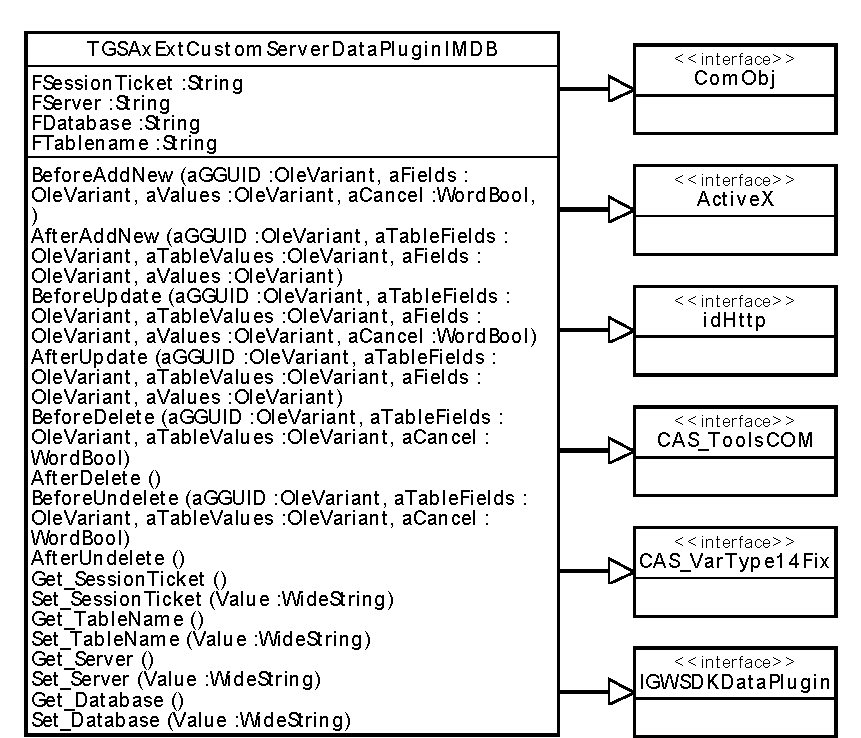
\includegraphics[scale=0.7]{pics/plugin_klassendiagramm.pdf}
\caption{Klassendiagramm Plugin}
\label{ergebniss_plugin_klassendiagramm}
\end{figure}

Die Funktionsweise wird im Folgenden anhand der Kommunikationen während einer Aktualisierung erläutert und in der Abbildung \ref{konzept_sequenz} dargestellt. Nachdem der Benutzer Datensätze geändert hat wird das Plugin aufgerufen. Die entsprechende Funktion erhält die \textit{GGUID} der Tupel, den Namen der Spalte, sowie die veränderten Werte. Anschließend wird überprüft, ob die Änderungen für unser System von Relevanz ist. Falls sie sich als relevant herausstellen, wird die \textit{aGGUID} in einen String konvertiert. Anschließend werden die Header-Werte der \textit{idHttp} Variable gesetzt. Sie beinhalten Werte wie die URI oder HTTP-Metadaten. Sobald alle Daten in der \textit{idHttp} gesetzt sind, wird ein POST-Request an unser System übermittelt. 

Der POST-Request enthält die \textit{GGUID} und die Art der Operation, die auf den Daten ausgeführt wurde. Bei neuen Daten beispielsweise wird ein Header namens "newGGUID" und dem Wert der \textit{GGUID} gesetzt. Im Anwendungsserver wird der neue Wert zuerst in eine CSV-Datei geschrieben und anschließend in die Datenbank eingefügt.


\begin{figure}[htbp]
\centering
  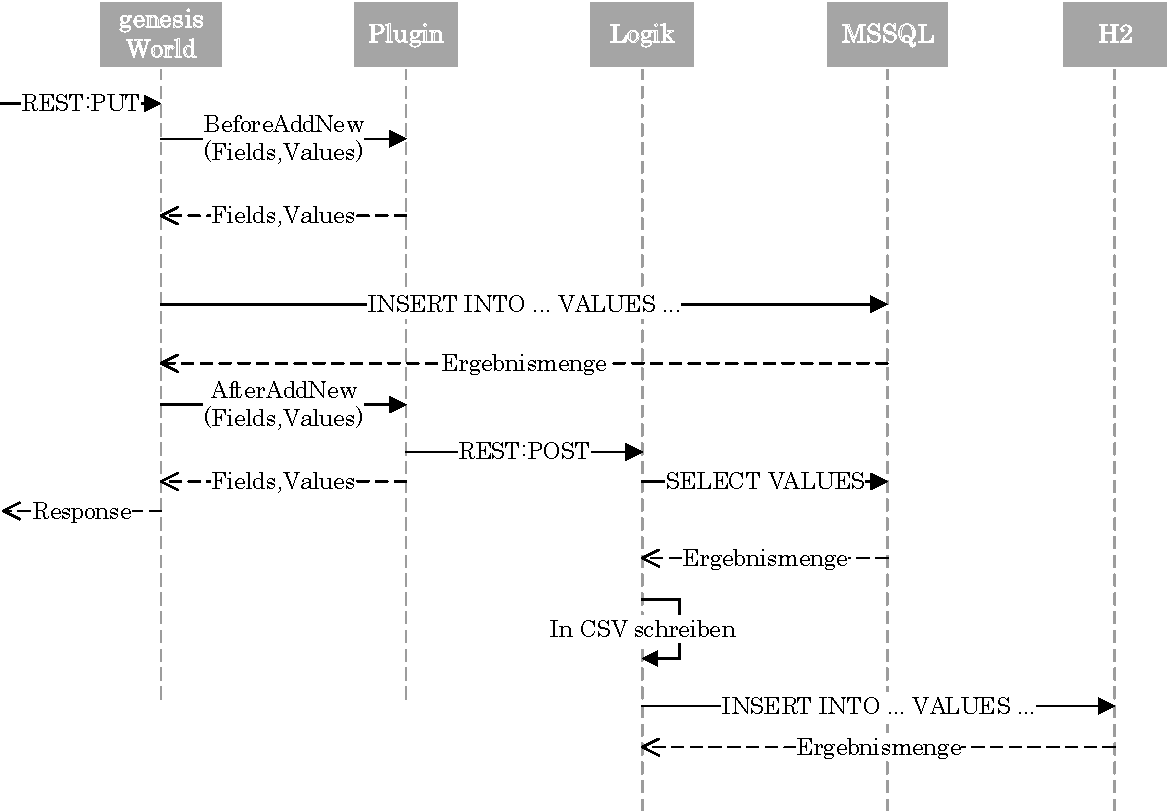
\includegraphics[width=0.8\textwidth]{pics/sequenzdiagramm.pdf}
\caption{Sequenzdiagramm für einen neuen Datensatz}
\label{konzept_sequenz}
\end{figure}



%% ===========================
\section{Oberfläche}
%% ===========================

In diesem Abschnitt wird die Umsetzung der Darstellung erörtert. Den Einstiegspunkt für Benutzer stellt das in Abbildung \ref{ergebniss_oberflaeche_anmeld} zu sehende Anmeldefenster dar. Der Hintergrund der Webseite ist in einem dunklen grau gestaltet, um einen Kontrast zum weißen Hintergrund der Bedienelemente zu schaffen. Zur Identifikation des Systems mit der Firma ist das Logo der CAS Software AG im linken Teil abgebildet. Im rechten Teil des Fensters existieren drei Eingabefelder. Zuerst ein Feld zur Eingabe der IP-Adresse des Server. Die dazugehörige Portnummer wird im darauf folgenden Feld eingegeben. Das dritte Feld ist für den Namen des Nutzers vorgesehen, der den Ausgangspunkt der Analyse darstellt. Abschließend wird ganz klassisch ein Button zum fortfahren auf der Webseite eingesetzt. Falls allerdings der eingegeben Nutzername nicht existiert, wird eine Warnmeldung direkt über dem zweiten Eingabefeld ausgegeben und auf der Anmeldeseite verblieben. 

\begin{figure}[htbp]
\centering
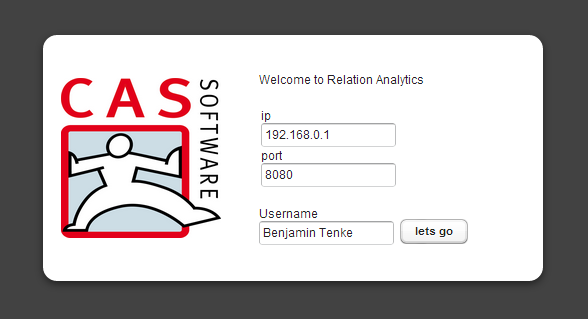
\includegraphics[scale=2.0]{pics/login.png}
\caption{Anmeldefenster}
\label{ergebniss_oberflaeche_anmeld}
\end{figure}

Das Hauptfenster wurde vom Aufbau, wie in Abschnitt \ref{ch:Konzeption:sec:Darstellungskonzepte} beschrieben umgesetzt. Im oberen Bereich befindet sich eine Leiste, die anhand der Microsoft Richtlinien für Design entworfen wurde. Dies schafft ein vertrautes Gefühl mit der Oberfläche und schafft eine schnelle Akzeptanz bei den Nutzern. Die Leiste ist in vier Bereiche aufgeteilt. Der erste Bereich, ganz links, dient der Gewichtung der Verbindungsmerkmale und dem anstoßen der Abfrage. Aufgrund der Gewichtung in Prozent, ist ein fester Wertebereich von 0 bis 100 vorgegeben. Textfelder eignen sich daher weniger, da sie beliebige Eingaben ermöglichen. Der Einsatz von Reglern bietet eine einfachere und selbsterklärende Form der Bedienung. Der begrenzte und kleine Wertebereich begünstigen den Einsatz der Regler. Zum stellen der Anfrage wird ein einfacher Button eingesetzt. Direkt unter dem Button befindet sich ein Text, der die benötigten Zeit für die Abfrage ausgibt. 

Der zweite Bereich dient zeitlichen Anpassungen. Das erste und dritte Feld können für Veränderung des Betrachtungszeitraums verwendet werden. Sie beinhalten den Anfangs- und Endzeitpunkt. Händische Eingaben weisen eine schlechte Bedienbarkeit auf, weswegen ein sogenannter "Datumspicker" eingesetzt wird. Dieser befindet sich direkt neben dem Textfeld und öffnet sich nach einem Klick auf das Symbol. Er stellt einen grafischen Kalender dar, aus dem durch klicken auf ein Tag das Datum bestimmt werden kann. Die Möglichkeit zur Eingabe durch direktes ändern des Textes bleibt allerdings weiterhin erhalten. Die anderen beiden Felder sind für die Gewichtung der Zeit vorgesehen. Diese Felder dienen zur Festlegung von $t_1$ und $t_2$, aus der Abbildung \ref{fig:umsetzung:gewichtungderzeit}. Das obere Feld ist für $t_1$. Hier kann die Zeitspanne zwischen $t_{s}$ und $t_1$ in Tagen festgelegt werden. Der Wert für die Zeitspanne zwischen $t_{e}$ und $t_2$ wird aus dem unteren Eingabefeld entnommen.

Bis auf den Achsschluss von Personen anhand ihrer Gruppen sind alle anderen Kriterien zur Filterungen der Personen im dritten Bereich vorhanden. Mithilfe der Checkboxen kann der Nutzer festlegen, welche Kriterien zum Ausschluss auf die Analyse angewendet werden sollten. Neben der Filterung durch bestimmte Personen, Länder, Städte usw. ist hier eine Begrenzung der Ergebnismenge umgesetzt. Im untersten Feld kann der Nutzer diese bestimmen.

Der Bereich ganz rechts in der Leiste, ist für den Ausschluss von Gruppen vorgesehen. Hier werden alle Gruppen im System mit einer Checkbox und einem Namen dargestellt. Dabei können beliebig viele Gruppen ausgewählt werden. Da die Anzahl der Gruppen überschaubar ist, entschied man sich alle anzuzeigen, anstatt einer händischen Eingabe der Namen durch den Nutzer. Für Benutzer entsteht dadurch ein Vorteil, da sie Gruppen auswählen können die sie zuvor nicht kannten.

\begin{figure}[htbp]
\centering
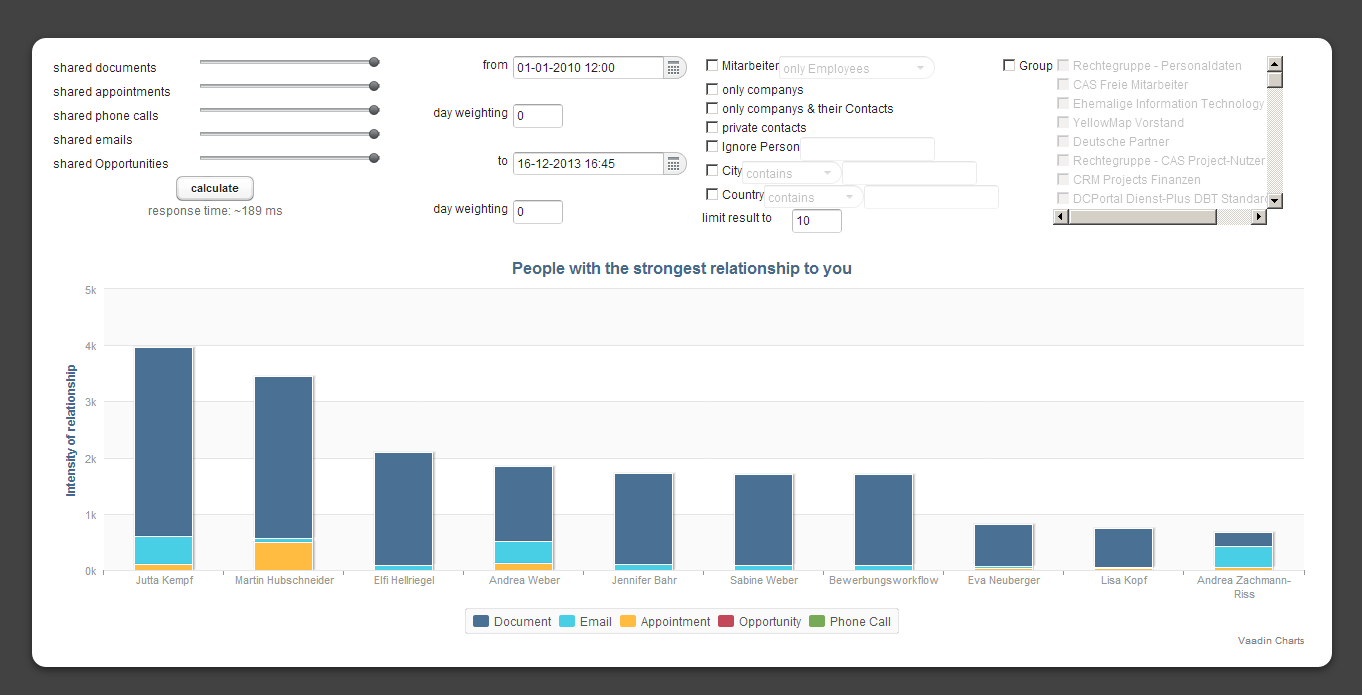
\includegraphics[width=\textwidth]{pics/final_screen.png}
\caption{Hauptseite der Anwendung}
\label{ergebniss_oberflaeche_haupt}
\end{figure}

Den zentralen Bereich des Fensters stellt das Diagramm dar. Die Balken selbst sind in fünf verschiedene Elemente unterteilt. Jedes Elemente wird durch eine andere Farbe dargestellt. Die fünf Elemente sind die verschiedenen CRM-Objekte. Die Zuordnung der Farbe zu dem jeweiligen Merkmal, wird über eine Legende im unteren Bereich des Fensters umgesetzt. Eine Besonderheit ist, dass durch einen Klick auf eine der Farben, das jeweilige Merkmal von der Darstellung ausgeschlossen wird. Beispielsweise kann der Nutzer auf die blaue Farbe neben dem Dokument klicken, was einen Neuaufbau des Diagramms ohne Dokumente bewirkt. Durch den Ausschluss wird allerdings keine neue Abfrage gesendet. Das  bedeutet die Reihenfolge in der die Personen angezeigt werden und die Datenbasis bleiben gleich. Mit einem wiederholten Klick auf die entsprechende Farbe in der Legende lässt sich der Originalzustand wiederherstellen. Zusätzlich zu der y-Achse, die eine Gesamtpunktzahl aufzeigt, kann der jeweilige Anteil eines Merkmals betrachtet werden. Dies geschieht durch einfaches platzieren des Mauszeigers, auf dem jeweiligen Bereich des Balkens. Dadurch öffnet sich ein Tooltip, welches die Anzahl der Punkte im Verhältnis zur Gesamtpunktzahl zeigt.

Die Ausführung der Anfrage erfolgt in der Regel mit dem dafür vorgesehen Button. Die Regler und das Datum, jedoch lösen bei Veränderungen automatisch eine neue Abfrage aus. Dies soll die hohe Antwortgeschwindigkeit des Systems untermalen und eine bessere Nutzererfahrung schaffen. Das Datum sowie die Gewichtung wurden dazu ausgewählt, da sie die am meisten benutzen Konfigurationsmöglichkeiten darstellen.

